\section{Implementation}
\label{sec:impl}

\sysname extends the LLVM compiler
infrastructure~\cite{llvm} and has three main components:
(1) a modified compiler frontend based on Clang~\cite{clang}
that augments C and C++ with an
approximation-aware type system;
(2) a program analysis and set of LLVM optimization passes that implement
program relaxations; and
(3) a feedback and autotuning system that automatically explores
quality--efficiency trade-offs.
% the fact that it's ``distributed'' doesn't matter yet

\subsection{Type System}

We implemented our approximation-aware type system, along with the syntactic
constructs \lil{APPROX} and \lil{ENDORSE}, as an extension to the Clang
C/C++ compiler.

\paragraph{Pluggable types layer.}

We modified Clang to support \emph{pluggable types} in the style of
Cqual~\cite{cqual} and Java's JSR-308 with its accompanying Checker
Framework~\cite{jsr308, papi}.
Pluggable types allow a compiler's built-in type system to be overlaid with
arbitrary qualifiers and typing rules. Syntactically, we
provide a GNU C \lil{__attribute__(())} construct that specifies the
type qualifiers for any variable, field, parameter, function, or method
definition. Our pluggable type library implements a bottom-up AST traversal
with an interface for defining typing rules.
Finally, the compiler emits LLVM IR bitcode
augmented with per-instruction metadata indicating the qualifiers on the
value of each SSA operation. For example, when the result of the
expression \lil{a + b} has the type \lil{APPROX float}, it emits an
\lil{add} instruction reflecting the qualifier. This
representation allows LLVM's compiler passes, which have access only to the IR
and not to the AST, to use the programmer-provided qualifier
information.
(We plan to release the source code for the generic
pluggable types layer along with the rest of the
system.)

% \xxx[br]{Explain why we don't need qualifier polymorphism, as explained in
% Section 18.2 of the Checker Framework manual.  Dan suggests we might make the
% subtle argument that approximate kernels don't touch much other code or use
% external libraries.}
% Despite Dan's suggestion, I think it's okay to omit polymorphism here.
% Bringing it up invites the criticism more than it assuages it, I think.
% -ALDS

\paragraph{Approximation-aware type system.}

The primary constructs in our EnerJ-inspired, approximation-aware type system
are the \lil{APPROX} type qualifier and the \lil{ENDORSE} explicit type
conversion. Both are provided as macros in a C header file. The
\lil{APPROX} macro expands to an \lil{__attribute__(())} construct,
and \lil{ENDORSE(e)} expands to an opaque C comma expression with a magic
number that the checker recognizes and interprets as a cast.
The type checker itself follows a standard information-flow implementation:
most expressions are approximate if any of their subexpressions is
approximate; \sysname checks types and emits errors in assignments, function
calls, function returns, and conditionals.

The escape hatches \annpermit and \annforbid are parsed from
C-style comments.

\subsection{Analysis and Relaxations}

\Precisepurity (\Sref{sec:precise-purity}) and region selection
(\Sref{subsec:regions}) are implemented as LLVM analysis passes. The \sysname
prototype includes three relaxations, also LLVM passes, that
consume the analysis results.
%
The \precisepurity analysis offers methods that check whether an individual LLVM
IR instruction is approximate, whether an instruction points to approximate
memory, and whether a code region (function or set of basic blocks) is \precisepure.
%
The region-selection analysis offers methods to enumerate \precisepure regions
of a function that can be treated specially, e.g., offloaded to an accelerator.

We special-case
the C memory-management intrinsics \lil{memcpy} and \lil{memset}
to assign them appropriate effects.
For example, \lil{memset(p,v,n)} where \lil{p} has type
\lil{APPROX float *} is
considered \precisepure because it behaves as a store to \lil{p}.

The loop-perforation and synchronization-elision relaxations
(\Sref{sec:relaxations}) use \precisepurity analysis to determine whether
a loop body or critical section can be considered approximate.
Loop perforation generates a counter and mask to skip iterations;
and synchronization elision deletes lock and barrier call instructions.
Neural acceleration uses region selection to identify target code and
subsequently generates inline ARM assembly to buffer data and communicate
with the FPGA over a coherent bus.

\subsection{Autotuning}

\sysname's autotuning system is implemented separately
from the compiler component. It communicates with the compiler via
command-line flags and a pass-generated configuration file that enumerates the
program's relaxation opportunities.

The programmer provides a quality metric to the autotuner in the form of a Python script that
defines a \lil{score} function, which
takes as input two execution outputs and
produces an error value between 0.0 and 1.0.

The autotuner's heuristic search consists of many independent program
executions, so it is embarrassingly parallel.
\sysname
optionally distributes the work across a cluster of machines to accelerate the
process.  Workers on each cluster node receive a configuration, compile the
program, execute it, and return the output and timing statistics. The master
node coordinates the search and reports results.

\subsection{Neural Acceleration}
\label{sec:accelerator}

We evaluate \sysname's approximate region selection using a Neural Processing
Unit (NPU) accelerator implemented on an on-chip FPGA (\Sref{sec:npu}).  The
design is based on recent work that implements an NPU based on systolic
arrays~\cite{npu, snnap}.

\iffalse
\begin{figure}
    \centering
    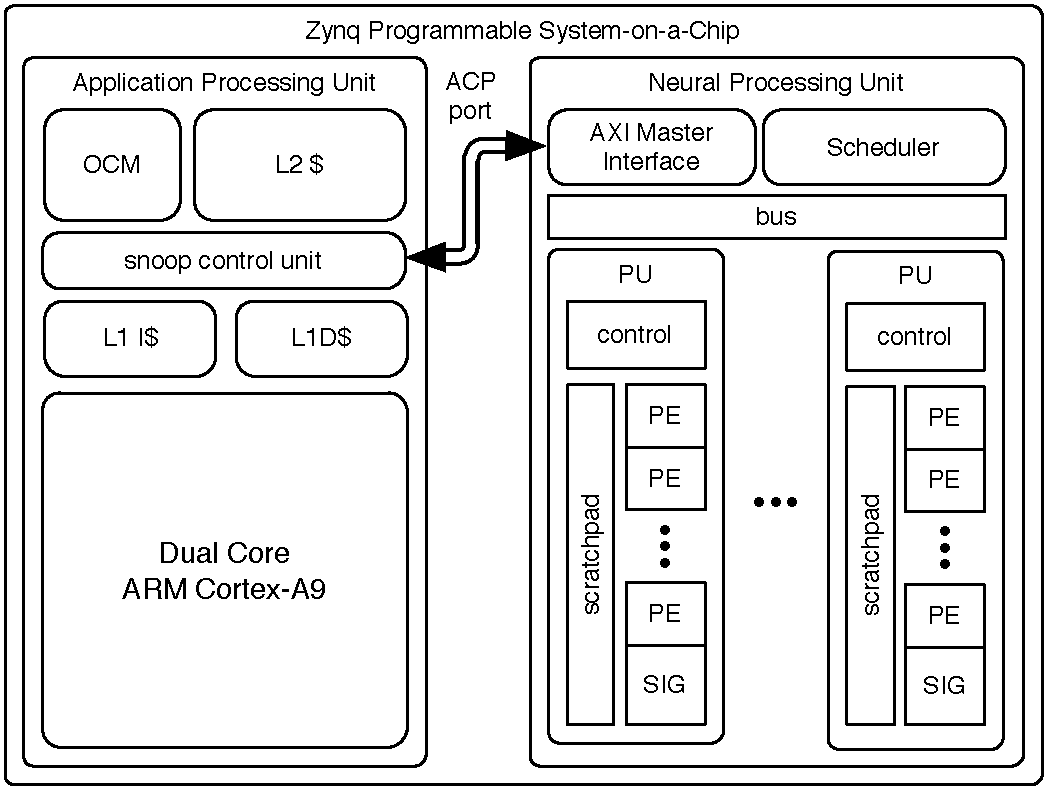
\includegraphics[width=0.8\linewidth]{figs/npu.pdf}
    \vspace{-1.5ex}
    \caption{Neural accelerator system diagram.}
    \label{fig:snnap}
\end{figure}

Our design, shown in  Figure~\ref{fig:snnap}, consists of a cluster of eight processing units (PUs) connected through a bus.
Each PU comprises a control block, a chain of processing elements (PEs),
and a sigmoid unit. The PEs are implemented on DSP logic and form a one-dimensional systolic array that feeds into
the sigmoid unit. When evaluating a neural network layer, PEs read the
synaptic weights from a scratchpad memory.
The sigmoid unit implements a nonlinear neuron-activation function
using a lookup table. At the core of the PU control block lies a configurable sequencer that
orchestrates communication between the PEs and the sigmoid unit. Different
PUs can be individually programmed to evaluate either a single or multiple different neural networks.

% 
% In its simplest form, the NPU is configured
% to accelerate the same neural network schedule across all eight PUs.
% 
% In this case, in order to orchestrate the parallel evaluation
% of neural networks, the NPU scheduler offloads the inputs to each PU in a round-robin fashion.

% Our FPGA-based NPU implementation has direct access to the snoop-control unit of the host processor through the
% accelerator coherency port (ACP). We designed a lightweight AXI master interface on the FPGA to read and write data to the
% processor's caches and on-chip memory (OCM). 

The NPU communicates with
the host processor through the accelerator coherency
port (ACP), which reads and writes data to the
processor's caches and on-chip memory (OCM). The host processor sends the neural network input sets to a region of the OCM that serves as a buffer. 
The host processor then signals the FPGA that the data is ready to be read using
the dedicated event-signaling instructions in
the ARMv7 ISA and transitions to a low-power state until it is awoken by the FPGA.
The FPGA reads the inputs
and evaluates the neural network. As results are generated, they are written back to the OCM, and once the NPU on the FPGA is
done processing the batch, it signals the host CPU that the output is ready. 

Full details on the FPGA design are out of the scope of this paper, since our
focus is on the programming framework, but will be made available in a technical
report after publication.
\fi
